\documentclass[12pt]{article}
\usepackage{amsmath}
\usepackage{geometry}
\usepackage{graphicx}
\usepackage{hyperref}
\usepackage[latin1]{inputenc}
\usepackage{listings}
\renewcommand{\labelitemi}{$\textendash$}
\geometry{
    a4paper,
    total={170mm,257mm},
    left=15mm,
    right=15mm,
    top=5mm,
    bottom=15mm
}

\title{CS4061: Week 4 Assignment}
\author{Conor McCauley - 17323203}
\date{November 4, 2020}

\begin{document}

\maketitle

\noindent \textbf{Dataset \#1 Identifier:} \texttt{\# id:13--13-13-0}

\noindent \textbf{Dataset \#2 Identifier:} \texttt{\# id:13--13--13-0}

\section*{Question (i)}

\noindent (a) We can first plot our dataset to get an idea of the data we're working with. The below plot show the input features along the x and y axes while the target value is plotted on the z-axis:

\begin{center}
    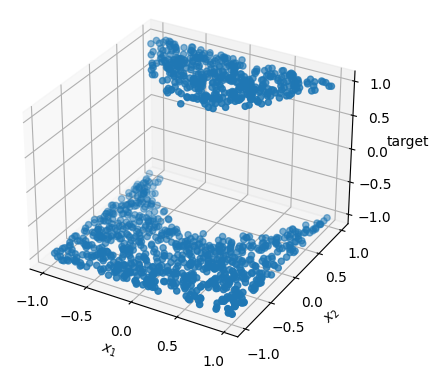
\includegraphics[scale=0.6]{fig_001.png}
\end{center}

From this plot alone it would appear that the training data is split along some two-dimensional curve.

In order to perform cross-validation using a logistic regression model we will need to select a range of $C$ penalties and a range of 'degree' values (the maximum order of polynomial features to add). Ideally, both of these ranges should, in all cases, contain examples of under-fitting at the lower values and examples of over-fitting at the higher values - this would imply that the optimal values lie within the chosen ranges.

By manually plotting the mean accuracy scores and standard deviations for wide ranges of $C$ ($10^{-4} - 10^{4}$) and degree ($1 - 7$) I was able to settle on the following suitable ranges for $C$ and degree (i.e. they contain both under-fitting and over-fitting):

\begin{center}
    \begin{tabular}{|c|c|}
        \hline
        $C$ &  $0.001, 0.01, 0.1, 1, 10, 100, 1000$ \\ \hline
        degree & $1, 2, 3, 4, 5, 6$ \\ \hline
    \end{tabular}
\end{center}

I chose to compare the trained models against two baseline models: one which always predicts the most frequent value and one which predicts random values. These models are generated using the following code:

\begin{center}
    \lstset{basicstyle=\footnotesize}
    \begin{lstlisting}[language=Python]
    bl_freq = DummyClassifier(strategy='most_frequent')
    bl_rand = DummyClassifier(strategy='uniform')
    \end{lstlisting}
\end{center}

When considering how many folds to use during cross-validation I settled on $k = 5$ as our dataset is not very large and it does not take up too much computation time. I also chose to measure the quality of our models using the 'accuracy' scoring method because we can also use this method for $k$NN in (b) and it allows us to compare our trained model against both baselines (using $F_1$ score would make our 'most frequent' baseline model useless as it would always score 0).

We can use the following code to run cross-validation for all of the models:

\begin{center}
    \lstset{basicstyle=\footnotesize}
    \begin{lstlisting}[language=Python]
    degree_rng = [1, 2, 3, 4, 5, 6]
    C_rng = [0.001, 0.01, 0.1, 1, 10, 100, 1000]
    for degree in degree_rng:
        X_poly = PolynomialFeatures(degree).fit_transform(X)
        for C in C_rng:
            model = LogisticRegression(C=C, penalty='l2', solver='lbfgs').fit(X_poly, Y)
            scores = cross_val_score(model, X_poly, Y, cv=5, scoring='accuracy')
    \end{lstlisting}
\end{center}

These models result in six different plots (one for each maximum polynomial degree). They are as follows:

\begin{center}
    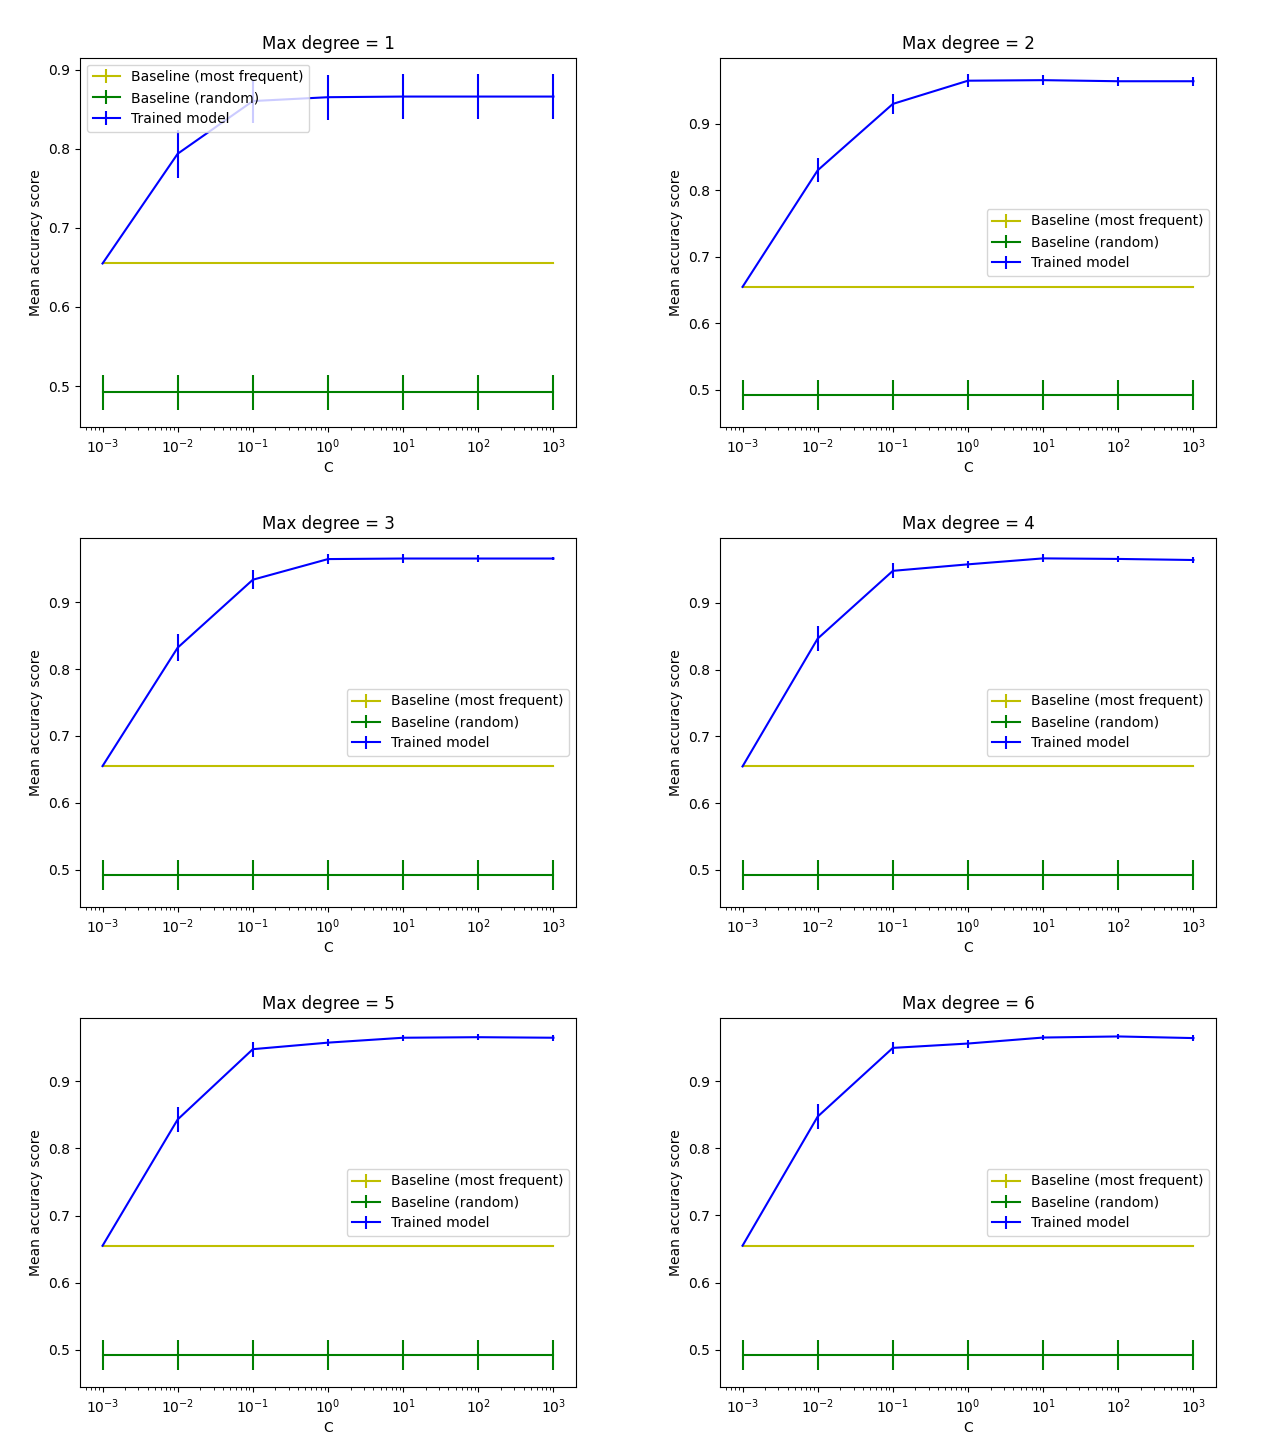
\includegraphics[scale=1.6]{fig_002.png}
\end{center}

From these plots we can see that, no matter what the value of degree is, we can dismiss all values of $C < 1$ as these $C$ values always have larger deviations and lower accuracy scores than values of $C \ge 1$. We can also dismiss the first plot (degree = 1) as it is clearly much less accurate than all subsequent models. For each remaining model all values of $C > 10$ represent minimal improvement over the scores reported for $C = 10$ and, as such, they can be dismissed.

The exact mean, $\mu$, and standard deviation, $\sigma$, values reported for $C \in \{1, 10\}$ and $2 \le$ degree $\le 6$ are as follows:

\begin{center}
    \begin{tabular}{|c|c|c|}
        \hline
        degree & $C = 1 \, (\mu, \sigma)$ & $C = 10 \, (\mu, \sigma)$ \\
        \hline
        $2$ &  $(0.965, 0.009)$ & $(0.966, 0.007)$ \\
        $3$ &  $(0.964, 0.007)$ & $(0.965, 0.006)$ \\
        $4$ &  $(0.958, 0.005)$ & $(0.967, 0.006)$ \\
        $5$ &  $(0.958, 0.005)$ & $(0.965, 0.004)$ \\
        $6$ &  $(0.956, 0.006)$ & $(0.965, 0.004)$ \\ \hline
    \end{tabular}
\end{center}

For each model $C = 10$ outperforms $C = 1$ as it has a higher accuracy and in all but one case it has a lower standard deviation. Finally, it seems that degree = 4 is the optimal degree value as it outperforms all lower degrees while maintaining a very small standard deviation. As such, we will use $C = 10$ and degree = 4.

We can generate a 2D array of values in the range $-3 \le x, y \le 3$ and use these values to examine how well a model using $C = 10$ and degree = 4 predicts values outside of the range of the training data. We can make these predictions using the following code:

\begin{center}
    \lstset{basicstyle=\footnotesize}
    \begin{lstlisting}[language=Python]
    X_pred = np.mgrid[-3:3.2:0.2, -3:3.2:0.2].reshape(2, -1).T
    X_pred_poly = PolynomialFeatures(degree).fit_transform(X_pred)
    Y_pred = model.predict(X_pred_poly)
    \end{lstlisting}
\end{center}

Plotting our predictions (blue) alongside our training data (red) produces the following graph:

\begin{center}
    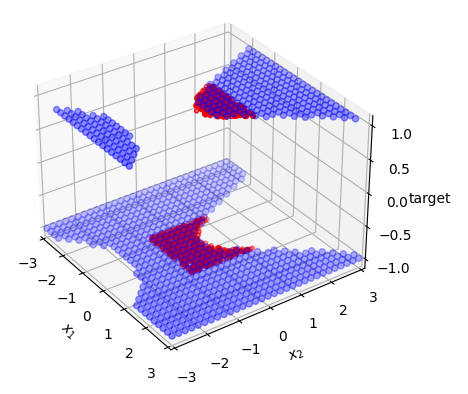
\includegraphics[scale=0.6]{fig_003.png}
\end{center}

Besides what appears to be a slight mirroring of the curve for lower values of $x_2$ the predictions are otherwise highly accurate!

\noindent (b) Before performing proper cross-validation on our models we will first investigate the effect of adding additional polynomial features to our dataset for a $k$NN model. We will again use 5-fold cross-validation and evaluate our models using the 'accuracy' scoring method for the reasons given in (a). We will also compare our trained model against a 'most frequent' baseline model and a 'random' baseline model. Using a broad range of $k$ values, $k \in \{3, 9, 15, 21\}$, and a decent range of degree values, degree $\in \{1, 2, 3, 4\}$, we can plot the mean accuracy score and standard deviation for each model. We can use the following code to do this:

\begin{center}
    \lstset{basicstyle=\footnotesize}
    \begin{lstlisting}[language=Python]
    k_rng = [3, 9, 15, 21]
    degree_rng = [1, 2, 3, 4]
    for k in k_rng:
        for degree in degree_rng:
            X_poly = PolynomialFeatures(degree).fit_transform(X)
            model = KNeighborsClassifier(n_neighbors=k, weights='uniform').fit(X_poly, Y)
            scores = cross_val_score(model, X_poly, Y, cv=5, scoring='accuracy')
    \end{lstlisting}
\end{center}

This results in the following plots:

\begin{center}
    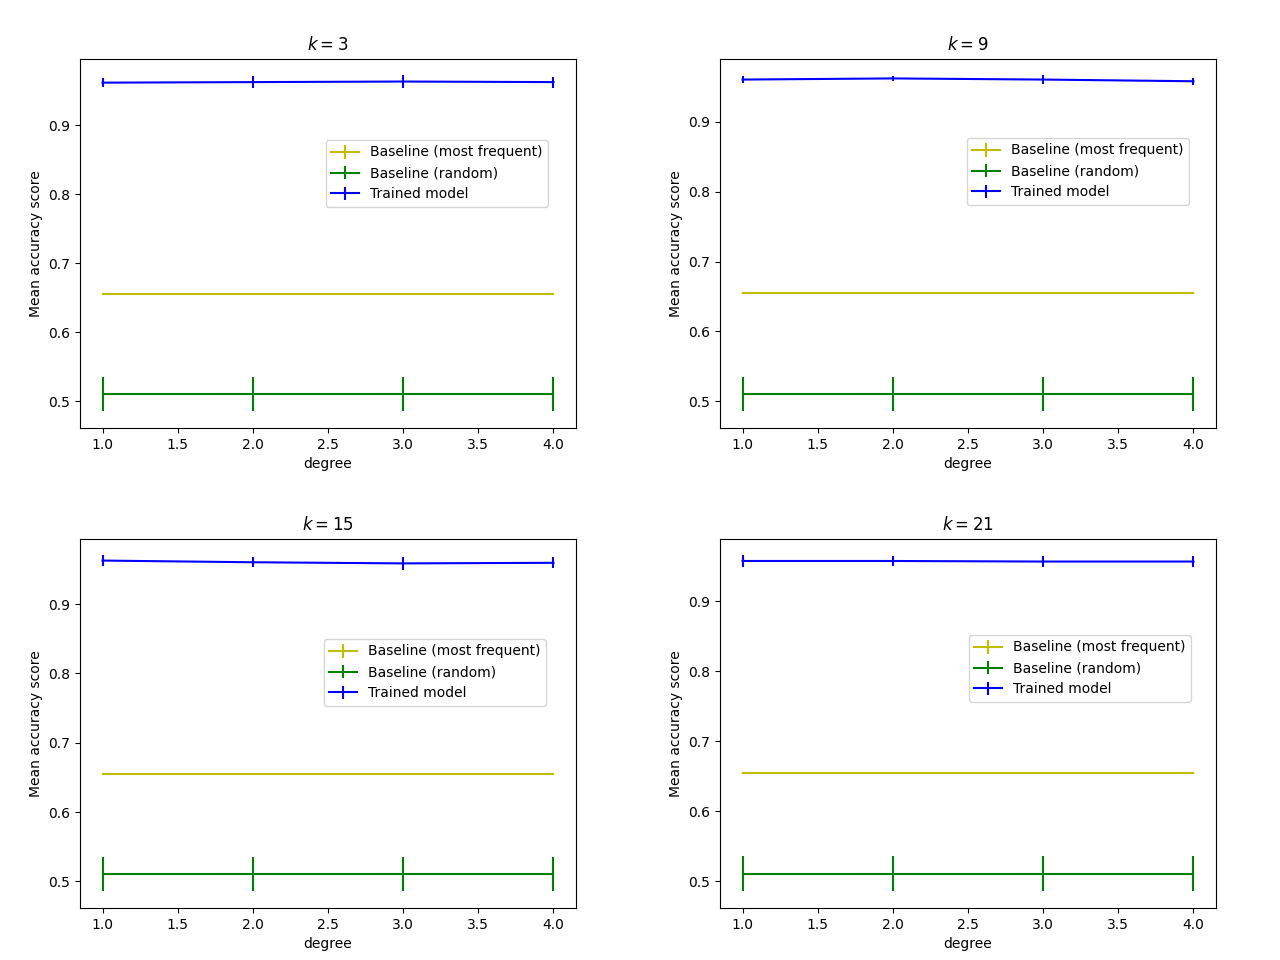
\includegraphics[scale=1.8]{fig_005.png}
\end{center}

It is clearly evident from the above plots that the addition of any number of polynomial features results in no improvement in the predictive accuracy of our $k$NN classifiers. As such, we will not make use of polynomial features in our final model.

We will first attempt to narrow down the range of ideal values of $k$ by plotting the mean accuracy score for a very broad and rough range of values, (i.e. $k \in \{5, 10, 25, 50, 100\}$. These values produce the following plot:

\begin{center}
    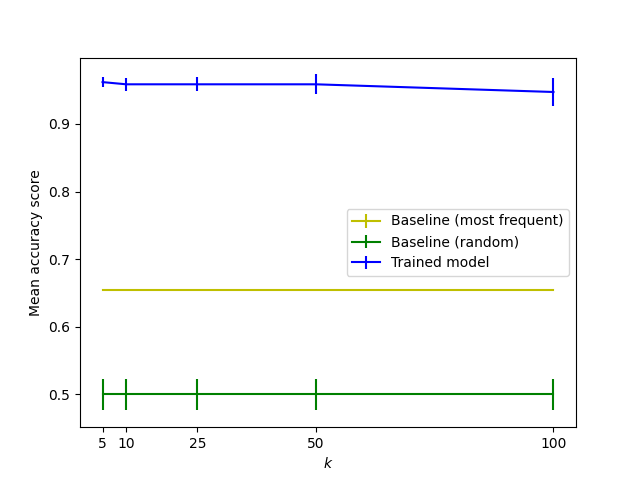
\includegraphics[scale=0.6]{fig_006.png}
\end{center}

Judging by these result it would seem that our optimal value of $k$ is less than 10. We can repeat this procedure with odd values in the range $3 \le k \le 11$ which results in the following plot:

\begin{center}
    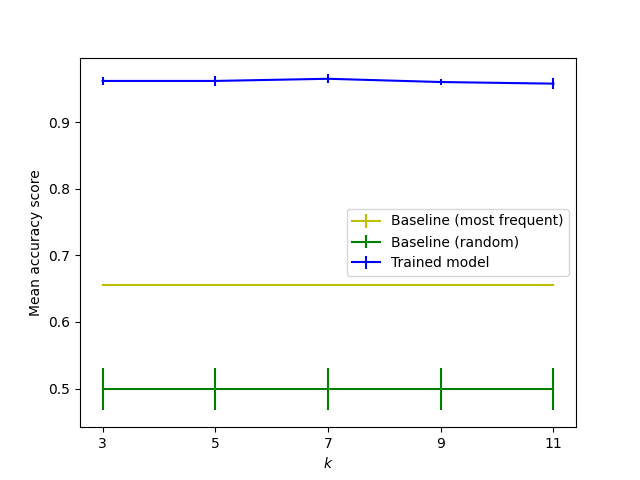
\includegraphics[scale=0.6]{fig_007.png}
\end{center}

Now, based on this plot it would appear that the optimal choice for $k$ is 7 as it performs slightly better than all the other values while having a very small standard deviation.

As in (a) we can test the quality of our resulting model by predicting values for features outside of the training data. Plotting our predictions (blue) alongside our training data (red) produces the following graph:

\begin{center}
    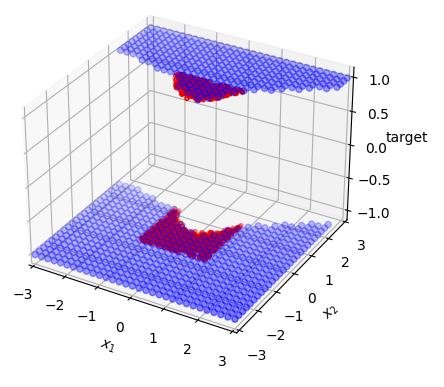
\includegraphics[scale=0.6]{fig_008.png}
\end{center}

These predictions are quite close to what we would expect given our training data, and, unlike with our logistic regression model, there are no anomalies in the predictions.

\noindent (c) For each of our models we can use the following code to calculate its confusion matrix (we use a \texttt{test\_size} value of $1 / k = 0.2$):

\lstset{basicstyle=\footnotesize}
\begin{lstlisting}[language=Python]
X_train, X_test, Y_train, Y_test = train_test_split(X, Y, test_size=0.2)
model = KNeighborsClassifier(n_neighbors=k, weights='uniform').fit(X_train, Y_train)
Y_pred = model.predict(X_test)
print(confusion_matrix(Y_test, Y_pred))
\end{lstlisting}

\noindent Our models produce the following confusion matrices: \\

Logistic regression model:

\begin{center}
    \begin{tabular}{c|c|c|}
        \hline
        true positive & 77 & 3 \\ \hline
        true negative & 1 & 166 \\ \hline
        & predict positive & predict negative \\
    \end{tabular}
\end{center}

$k$NN model:

\begin{center}
    \begin{tabular}{c|c|c|}
        \hline
        true positive & 81 & 7 \\ \hline
        true negative & 4 & 155 \\ \hline
        & predict positive & predict negative \\
    \end{tabular}
\end{center}

Baseline model (most frequent):

\begin{center}
    \begin{tabular}{c|c|c|}
        \hline
        true positive & 0 & 94 \\ \hline
        true negative & 0 & 153 \\ \hline
        & predict positive & predict negative \\
    \end{tabular}
\end{center}

Baseline model (random):

\begin{center}
    \begin{tabular}{c|c|c|}
        \hline
        true positive & 45 & 49 \\ \hline
        true negative & 80 & 73 \\ \hline
        & predict positive & predict negative \\
    \end{tabular}
\end{center}

We can see from these matrices that our logistic regression model makes accurate prediction for over 98\% of the test data which is slightly better than the 95.5\% accuracy rate of our $k$NN model. Neither of our baseline models perform very well compared to our trained models although our 'most frequent' baseline is a good deal more accurate than our 'random' baseline.

\noindent (d) We can use the following code to plot the ROC curves of our models:

\begin{center}
    \lstset{basicstyle=\footnotesize}
    \begin{lstlisting}[language=Python]
    lr_fpr, lr_tpr, _ = roc_curve(Y_test, lr_model.decision_function(X_test))
    knn_fpr, knn_tpr, _ = roc_curve(Y_test, knn_model.predict_proba(X_test)[:, 1])
    \end{lstlisting}
\end{center}

These plots (which include points for each of our baseline models) are as follows:

\begin{center}
    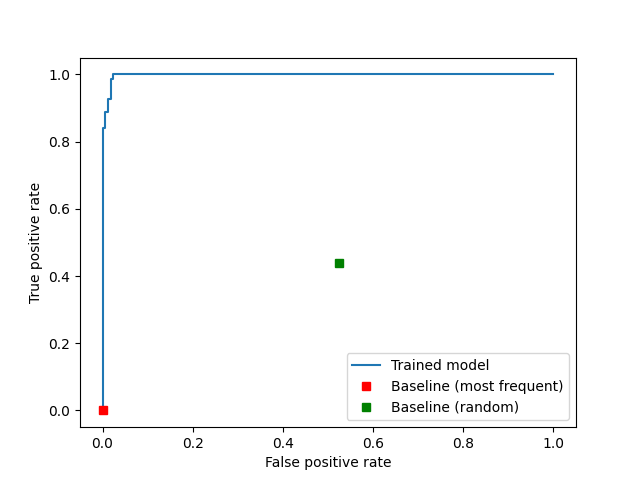
\includegraphics[scale=0.6]{fig_009.png}
    
    ROC curve for logistic regression model
    
    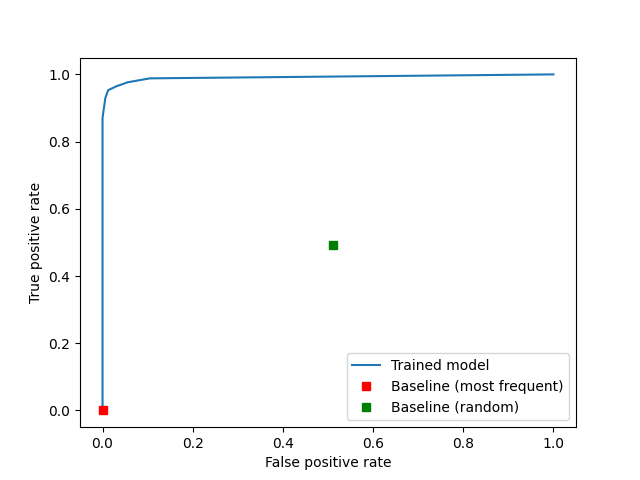
\includegraphics[scale=0.6]{fig_010.png}
    
    ROC curve for $k$NN model
\end{center}

In both cases, due to the high predictive accuracy of our models, the ROC curves tend to remain very close to the top left indicating a very high true positive rate (as mentioned in (c)).

Due to fact that the most frequent target value is -1 it is to be expected that a 'most frequent' baseline classifier (which will always predict -1) will have a true positive rate of 0 - this can be seen in both plots.

Our 'random' baseline classifiers both lie directly in the middle of our plots due to the fact that it's equally likely to correctly or incorrectly predict a positive target value leading to both a true and false positive rate of approximately 0.5.

\noindent (e) As mentioned in (c) and (d) and as was clearly evident from our plots in (a) and (b) both of our trained models vastly outperform our baseline classifiers. Looking at the ROC curves from (d) it is very clear that our trained models have much better true positive rates when compared to our 'random' baseline classifier (as discussed in (d)).

From (c) we can see that our logistic regression model is, overall, slightly more accurate than our $k$NN model. The true positive rate of our logistic regression model (96\%) is also a good deal higher than the true positive rate of our $k$NN model (92\%). These results would seem to indicate that the logistic regression classifier is a better choice than our $k$NN classifier. However, when we predicted values for an extended range of input features our logistic regression model resulted in some apparently inaccurate predictions for low values of $x_2$. In contrast, our $k$NN model did not make similar inaccurate predictions (although our logistic regression model appeared to make slightly more accurate predictions than our $k$NN model for basically all other values of $x_2$).

Considering all of the above I would probably recommend the logistic regression classifier due to its better predictive accuracy while keeping in mind that it may not scale well with certain data outside of the range $-1 \le x_1, x_2 \le 1$. However, given that our $k$NN classifier is also quite accurate and appears to scale well with unseen data it would not be a particularly bad choice either (although preference is given to the logistic regression classifier).

\section*{Question (ii)}

\textbf{N.B.} as the code used in this question is identical to the code used in (i) I will not repeat any code explanation nor provide additional code snippets. \\

\noindent (a) As in (i), we can first plot our dataset:

\begin{center}
    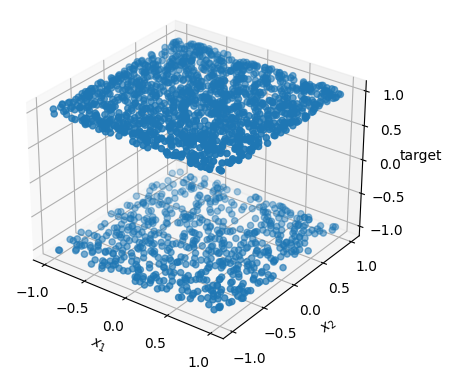
\includegraphics[scale=0.6]{fig_101.png}
\end{center}

Judging from this plot there does not seem to be any obvious pattern in how target values are chosen. It would appear that target values are randomly selected (with a bias towards +1).

Using the same method as in (i) I narrowed down the potential ranges of $C$ and degree and settled on the following ranges (although practically all combinations of $C$ and degree led to the same poor predictive results given the apparent randomness of the dataset):

\begin{center}
    \begin{tabular}{|c|c|}
        \hline
        $C$ &  $0.1, 1, 10, 100, 1000, 10000$ \\ \hline
        degree & $1, 3, 5, 7$ \\ \hline
    \end{tabular}
\end{center}

I once again chose to use 5-fold cross-validation as well as the 'accuracy' scoring method for the same reasons I gave in (i). I also chose to compare our predictions against the same two baseline models. Our models produce the following four plots:

\begin{center}
    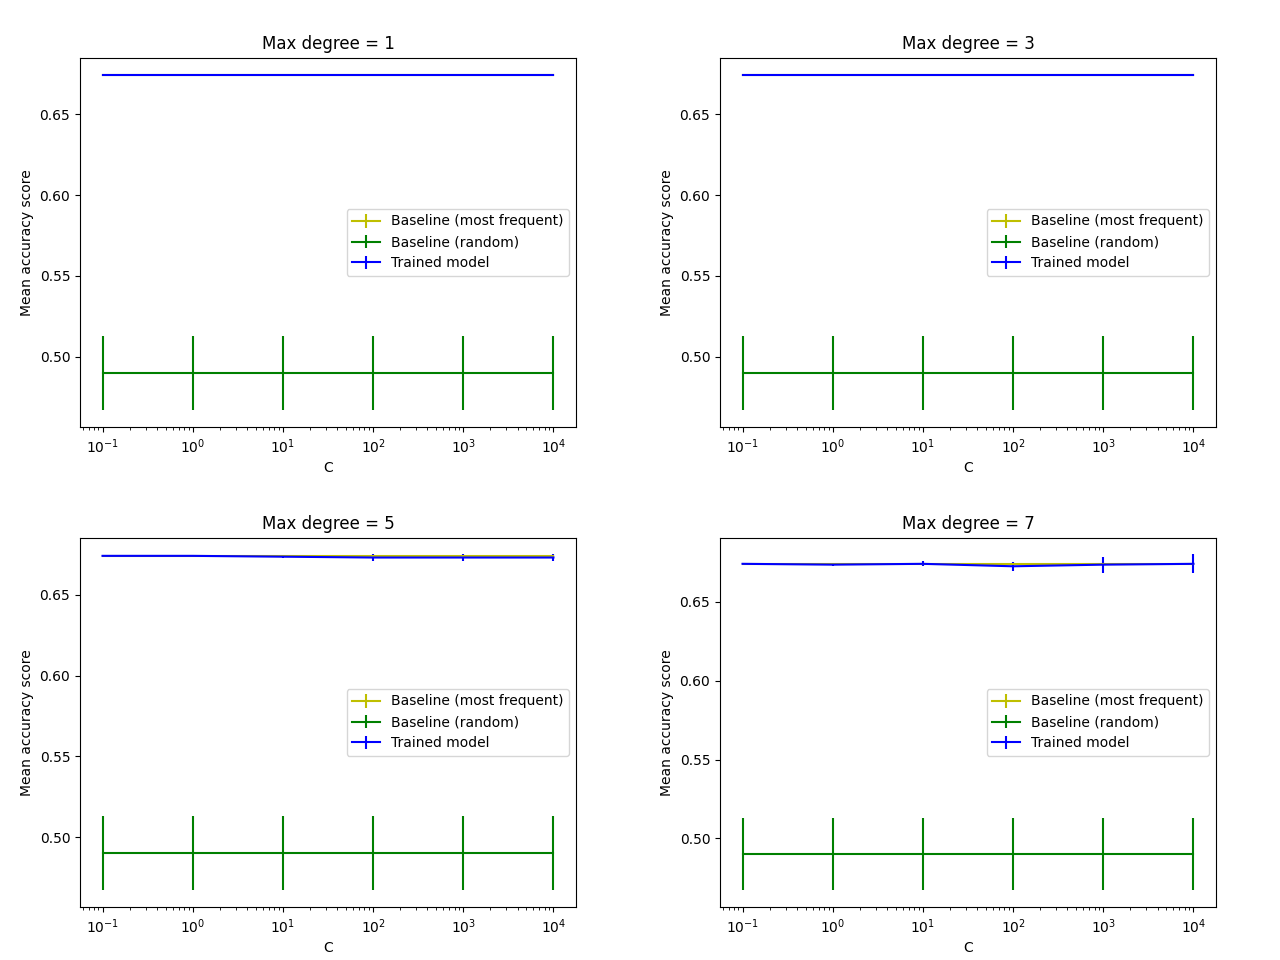
\includegraphics[scale=1.8]{fig_102.png}
\end{center}

No combination of $C$ and degree outperforms our 'most frequent' baseline model and higher values of degree actually lead to models that perform worse than the baseline. As such, there is no apparent reason for us to add any additional polynomial features nor should we use a non-standard value of $C$. We will use degree = 1 and $C = 1$.

As in (i) we can generate range of feature values outside the range of the training data and visualise our models predictions. Plotting our predictions (blue) alongside our training data (red) produces the following graph:

\begin{center}
    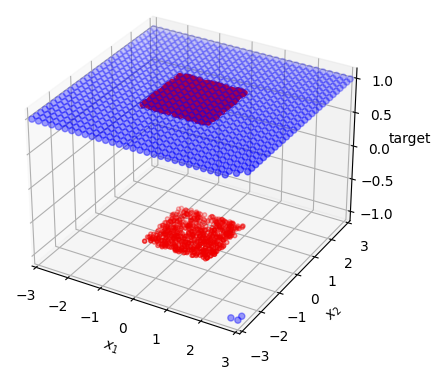
\includegraphics[scale=0.6]{fig_103.png}
\end{center}

Unsurprisingly, our model predicts +1 in practically all cases (I'm not entirely sure why for very low values of both $x_1$ and $x_2$ the model predicts -1 but this anomaly does not have much of an effect on the overall results).

\noindent (b) As in (i) we can investigate the effect of adding additional polynomial features to our dataset using the same range of $k$ values and degree values. We get the following plots:

\begin{center}
    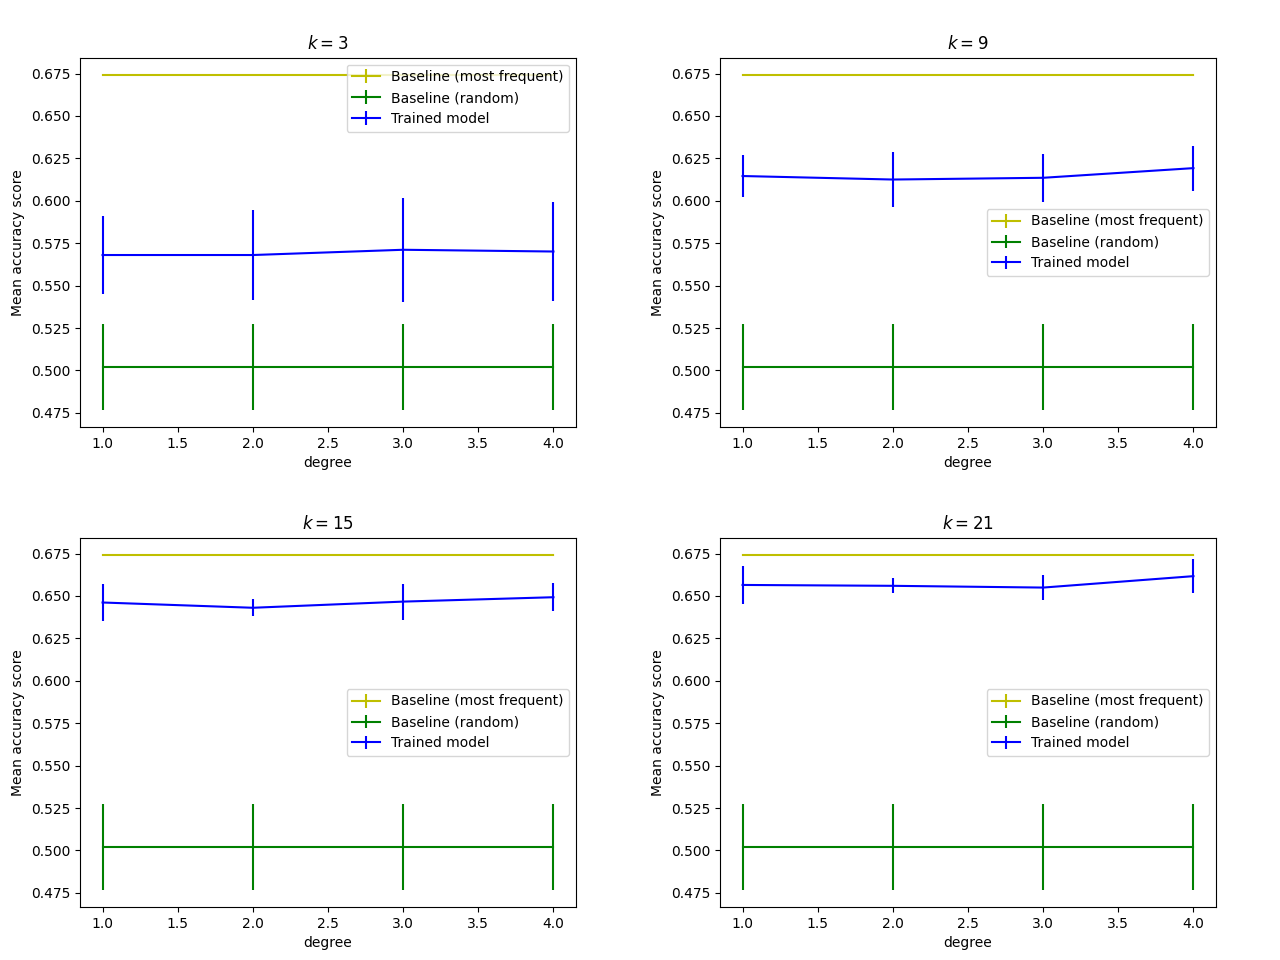
\includegraphics[scale=1.8]{fig_105.png}
\end{center}

Again, it appears that there is no significant improvement in the predictive accuracy of any of our models by adding additional polynomial features, and as such, we will not use them.

As in (i) we will use first use a broad range of $k$ values, $k \in \{5, 10, 25, 50, 100\}$, in order to get a rough idea of where the optimal $k$ value lies. We get the following plot:

\begin{center}
    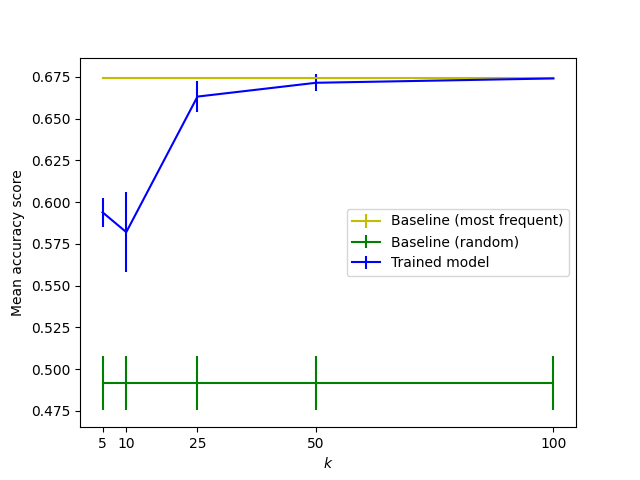
\includegraphics[scale=0.6]{fig_106.png}
\end{center}

This result is not unexpected. Given that higher values of $k$ lead to under-fitting and that the optimal model for this dataset is simply to always predict +1 it makes sense that the higher the value of $k$ the more accurate our model is - although it will never outperform our 'most frequent' baseline. As such, we can use $k = 100$ (although any similar large value of $k$ would work just as well).

Plotting predictions (blue) for an extended range of feature values alongside our training data (red) produces the following graph:

\begin{center}
    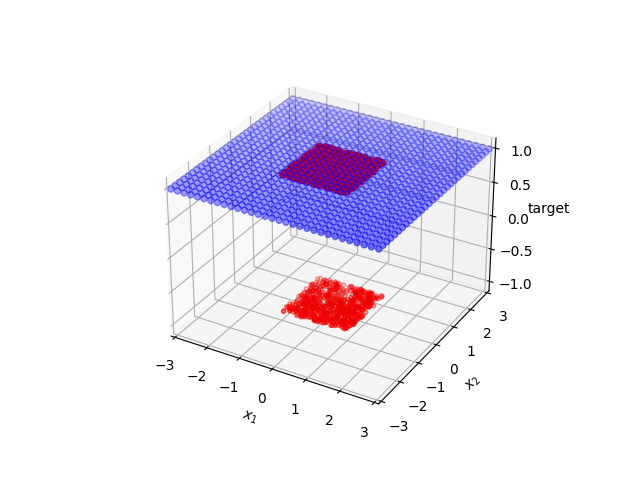
\includegraphics[scale=0.6]{fig_107.png}
\end{center}

\noindent (c) As in (i) we can generate confusion matrices for each of our models: \\

Logistic regression model:

\begin{center}
    \begin{tabular}{c|c|c|}
        \hline
        true positive & 247 & 0 \\ \hline
        true negative & 140 & 0 \\ \hline
        & predict positive & predict negative \\
    \end{tabular}
\end{center}

$k$NN model:

\begin{center}
    \begin{tabular}{c|c|c|}
        \hline
        true positive & 263 & 0 \\ \hline
        true negative & 124 & 0 \\ \hline
        & predict positive & predict negative \\
    \end{tabular}
\end{center}

Baseline model (most frequent):

\begin{center}
    \begin{tabular}{c|c|c|}
        \hline
        true positive & 266 & 0 \\ \hline
        true negative & 121 & 0 \\ \hline
        & predict positive & predict negative \\
    \end{tabular}
\end{center}

Baseline model (random):

\begin{center}
    \begin{tabular}{c|c|c|}
        \hline
        true positive & 138 & 128 \\ \hline
        true negative & 61 & 60 \\ \hline
        & predict positive & predict negative \\
    \end{tabular}
\end{center}

Due to the apparent randomness of the training data neither of our trained models perform any better than our 'most frequent' baseline model. This is because both of our models are essentially acting as 'most frequent' classifiers. Our $k$NN model is slightly more accurate than our logistic regression model (68\% vs. 64\%) while our 'most frequent' baseline actually outperforms our trained models slightly with an accuracy of 69\%. Our 'random' baseline model performs very poorly, which is expected given how many more +1 target values there are than -1 values.

\noindent (d) As in (i) we can plot the ROC curves of each of our models along with the points of each of our baseline models:

\begin{center}
    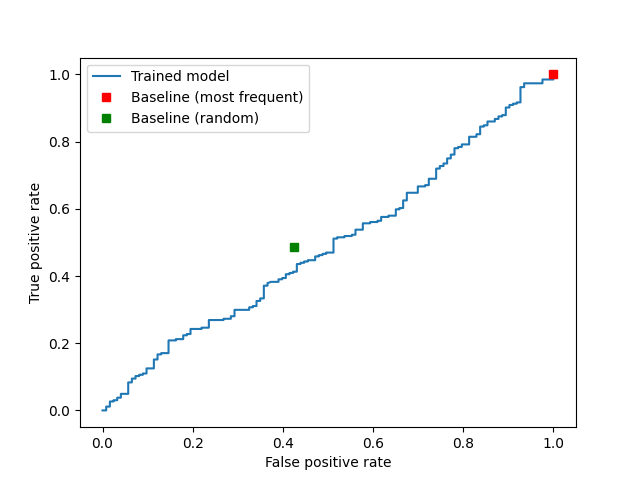
\includegraphics[scale=0.6]{fig_108.png}
    
    ROC curve for logistic regression model
    
    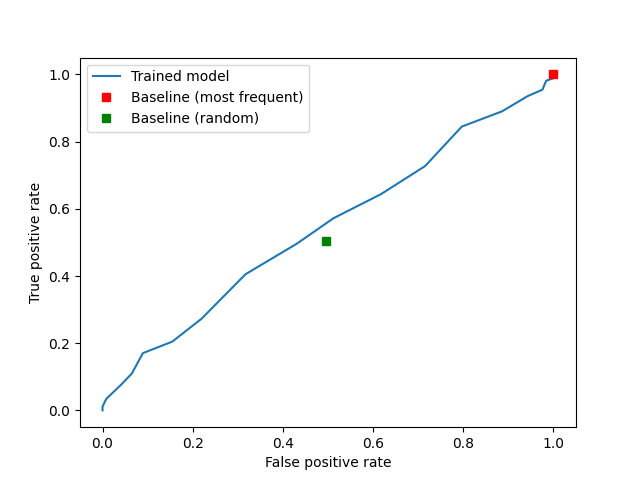
\includegraphics[scale=0.6]{fig_109.png}
    
    ROC curve for $k$NN model
\end{center}

As explained in (i) our 'random' baseline classifiers both lie directly in the middle of our plots due to the fact that it's equally likely to correctly or incorrectly predict a positive target value leading to both a true and false positive rate of approximately 0.5.

Both of our trained models have true positive rates proportional to the number of target values that are +1 since they always predict +1. This same effect can be seen with our 'most frequent' baseline model.

\noindent (e) As we saw from our plots in (a) and (b) as well as our matrices in (c) neither of our trained models were able to achieve a higher accuracy than that of our 'most frequent' baseline model. In fact, our trained models were slightly less accurate than our 'most frequent' baseline model in some cases. As mentioned in (d) the ROC curves for each of our trained models are very similar to those of our 'random' classifier which indicates that they are pretty much useless as predictive models.

For this dataset I would simply recommend the 'most frequent' baseline model for two reasons: it performs better than or equal to our trained models and it requires very little computation to make predictions unlike our trained models which are essentially just needlessly wasting computational time.

\section*{Appendix: Code}

\lstset{basicstyle=\footnotesize}
\begin{lstlisting}[language=Python]
from matplotlib import cm
from mpl_toolkits.mplot3d import Axes3D
from sklearn.dummy import DummyClassifier
from sklearn.linear_model import LogisticRegression
from sklearn.metrics import confusion_matrix, roc_curve
from sklearn.model_selection import cross_val_score, train_test_split
from sklearn.neighbors import KNeighborsClassifier
from sklearn.preprocessing import PolynomialFeatures
import matplotlib.pyplot as plt
import numpy as np
import pandas as pd
import warnings

# suppress SciKit warnings
warnings.filterwarnings('ignore')

# select specific feature from the data
def filter_data(data, index):
    return [d[index] for d in data]

# reshape data into X and Y arrays
def reshape_data(data):
    X1 = np.array(filter_data(data, 0)).reshape(-1, 1)
    X2 = np.array(filter_data(data, 1)).reshape(-1, 1)
    X = np.column_stack((X1, X2))
    Y = np.array(filter_data(data, 2))
    return X, Y

# plot only the dataset
def plot_dataset(data):
    X = filter_data(data, 0)
    Y = filter_data(data, 1)
    Z = filter_data(data, 2)
    fig = plt.figure()
    ax = fig.add_subplot(111, projection='3d')
    ax.scatter(X, Y, Z)
    ax.set_xlabel('$x_1$')
    ax.set_ylabel('$x_2$')
    ax.zaxis.set_rotate_label(False)
    ax.set_zlabel('target', rotation=0)
    plt.show()

# plot dataset with predictions
def plot_dataset_with_predictions(data, pred_data, pred_results):
    fig = plt.figure()
    ax = fig.add_subplot(111, projection='3d')
    # plot predictions
    X1 = filter_data(pred_data, 0)
    X2 = filter_data(pred_data, 1)
    ax.scatter(X1, X2, pred_results, c='#0000ff80')
    # plot training data
    X = filter_data(data, 0)
    Y = filter_data(data, 1)
    Z = filter_data(data, 2)
    ax.scatter(X, Y, Z, c='#ee000088', edgecolors='#ee0000', s=8)
    # configure and show plot
    ax.zaxis.set_rotate_label(False)
    ax.set_xlabel('$x_1$')
    ax.set_ylabel('$x_2$')
    ax.set_zlabel('target', rotation=0)
    ax.set_xlim3d(-3, 3)
    ax.set_ylim3d(-3, 3)
    plt.show()

# logistic regression: cross-val, plotting, matrices, ROC, ...
def logistic_regression(data, set_num):
    # reshape data
    X, Y = reshape_data(data)
    
    # initialise baseline models and get scores
    bl_freq = DummyClassifier(strategy='most_frequent')
    bl_freq_scores = cross_val_score(bl_freq, X, Y, cv=5, scoring='accuracy')
    bl_freq_mean, bl_freq_std = bl_freq_scores.mean(), bl_freq_scores.std()
    bl_rand = DummyClassifier(strategy='uniform')
    bl_rand_scores = cross_val_score(bl_rand, X, Y, cv=5, scoring='accuracy')
    bl_rand_mean, bl_rand_std = bl_rand_scores.mean(), bl_rand_scores.std()
    
    # initialise ranges
    if set_num == 1:
        degree_rng = [1, 2, 3, 4, 5, 6]
        C_rng = [0.001, 0.01, 0.1, 1, 10, 100, 1000]
    else:
        degree_rng = [1, 3, 5, 7]
        C_rng = [0.1, 1, 10, 100, 1000, 10000]
    
    # run cross-validation on all models
    for degree in degree_rng:
        X_poly = PolynomialFeatures(degree).fit_transform(X)
        means, stds = [], []
        for C in C_rng:
            model = LogisticRegression(C=C, penalty='l2', solver='lbfgs').fit(X_poly, Y)
            scores = cross_val_score(model, X_poly, Y, cv=5, scoring='accuracy')
            means.append(scores.mean())
            stds.append(scores.std())
        # output relevant data
        print('\ndegree = %d:' % (degree))
        for i, C in enumerate(C_rng):
            print('C = %.3ff >> mean = %.3f, std = %.3f' % (C, means[i], stds[i]))
        # extend baseline values into arrays
        bl_freq_means = [bl_freq_mean] * len(C_rng)
        bl_freq_stds = [bl_freq_std] * len(C_rng)
        bl_rand_means = [bl_rand_mean] * len(C_rng)
        bl_rand_stds = [bl_rand_std] * len(C_rng)
        # plot mean and std deviation for each C along with baselines
        plt.errorbar(C_rng, bl_freq_means, yerr=bl_freq_stds, fmt='y')
        plt.errorbar(C_rng, bl_rand_means, yerr=bl_rand_stds, fmt='g')
        plt.errorbar(C_rng, means, yerr=stds, fmt='b')
        plt.xlabel('C')
        plt.ylabel('Mean accuracy score')
        plt.xscale('log')
        plt.legend(['Baseline (most frequent)', 'Baseline (random)', 'Trained model'])
        plt.title(f'Max degree = {degree}')
        plt.show()
    
    # initialise optimal values
    if set_num == 1:
        degree = 4
        C = 10
    else:
        degree = 1
        C = 1

    # train model and calculate confusion matrix
    X_poly = PolynomialFeatures(degree).fit_transform(X)
    X_train, X_test, Y_train, Y_test = train_test_split(X_poly, Y, test_size=0.2)
    model = LogisticRegression(C=C, penalty='l2', solver='lbfgs').fit(X_train, Y_train)
    Y_pred = model.predict(X_test)
    print(confusion_matrix(Y_test, Y_pred))

    # make predictions for an extended range of feature values
    X_pred = np.mgrid[-3:3.2:0.2, -3:3.2:0.2].reshape(2, -1).T
    X_pred_poly = PolynomialFeatures(degree).fit_transform(X_pred)
    plot_dataset_with_predictions(data, list(X_pred), list(model.predict(X_pred_poly)))

    # calculate confusion matrices for both baselines
    bl_X_train, bl_X_test, bl_Y_train, bl_Y_test = train_test_split(X, Y, test_size=0.2)
    bl_freq.fit(bl_X_train, bl_Y_train)
    bl_freq_pred = bl_freq.predict(bl_X_test)
    bl_freq_cm = confusion_matrix(bl_Y_test, bl_freq_pred)
    print(bl_freq_cm)
    bl_rand.fit(bl_X_train, bl_Y_train)
    bl_rand_pred = bl_rand.predict(bl_X_test)
    bl_rand_cm = confusion_matrix(bl_Y_test, bl_rand_pred)
    print(bl_rand_cm)

    # ROC curve with baseline points
    fpr, tpr, _ = roc_curve(Y_test, model.decision_function(X_test))
    plt.plot(fpr, tpr)
    bl_freq_tpr = bl_freq_cm[1][1] / (bl_freq_cm[1][1] + bl_freq_cm[1][0])
    bl_freq_fpr = bl_freq_cm[0][1] / (bl_freq_cm[0][1] + bl_freq_cm[0][0])
    plt.plot(bl_freq_fpr, bl_freq_tpr, 'rs')
    bl_rand_tpr = bl_rand_cm[1][1] / (bl_rand_cm[1][1] + bl_rand_cm[1][0])
    bl_rand_fpr = bl_rand_cm[0][1] / (bl_rand_cm[0][1] + bl_rand_cm[0][0])
    plt.plot(bl_rand_fpr, bl_rand_tpr, 'gs')
    plt.xlabel('False positive rate')
    plt.ylabel('True positive rate')
    plt.legend(['Trained model', 'Baseline (most frequent)', 'Baseline (random)'])
    plt.show()

# kNN: cross-val, plotting, matrices, ROC, ...
def knn(data, set_num):
    # reshape data
    X, Y = reshape_data(data)
    
    # initialise baseline models and get scores
    bl_freq = DummyClassifier(strategy='most_frequent')
    bl_freq_scores = cross_val_score(bl_freq, X, Y, cv=5, scoring='accuracy')
    bl_freq_mean, bl_freq_std = bl_freq_scores.mean(), bl_freq_scores.std()
    bl_rand = DummyClassifier(strategy='uniform')
    bl_rand_scores = cross_val_score(bl_rand, X, Y, cv=5, scoring='accuracy')
    bl_rand_mean, bl_rand_std = bl_rand_scores.mean(), bl_rand_scores.std()
    
    # initialise ranges
    if set_num == 1:
        degree_rng = [1, 2, 3, 4]
        k_rng = [3, 7, 11, 15, 19, 23, 27, 31, 35, 39]
    else:
        degree_rng = [1, 2, 3, 4]
        k_rng = [3, 7, 11, 15, 19, 23, 27, 31, 35, 39]
    
    # run cross-validation to test effect of polynomial features
    for k in [3, 9, 15, 21]:
        means, stds = [], []
        for degree in degree_rng:
            X_poly = PolynomialFeatures(degree).fit_transform(X)
            model = KNeighborsClassifier(n_neighbors=k, weights='uniform').fit(X_poly, Y)
            scores = cross_val_score(model, X_poly, Y, cv=5, scoring='accuracy')
            means.append(scores.mean())
            stds.append(scores.std())
        # output relevant data
        print('\nk = %d:' % (k))
        for i, degree in enumerate(degree_rng):
            print('degree = %d >> mean = %.3f, std = %.3f' % (degree, means[i], stds[i]))
        # extend baseline values into arrays
        bl_freq_means = [bl_freq_mean] * len(degree_rng)
        bl_freq_stds = [bl_freq_std] * len(degree_rng)
        bl_rand_means = [bl_rand_mean] * len(degree_rng)
        bl_rand_stds = [bl_rand_std] * len(degree_rng)
        # plot mean and std deviation for each C along with baselines
        plt.errorbar(degree_rng, bl_freq_means, yerr=bl_freq_stds, fmt='y')
        plt.errorbar(degree_rng, bl_rand_means, yerr=bl_rand_stds, fmt='g')
        plt.errorbar(degree_rng, means, yerr=stds, fmt='b')
        plt.xlabel('degree')
        plt.ylabel('Mean accuracy score')
        plt.legend(['Baseline (most frequent)', 'Baseline (random)', 'Trained model'])
        plt.title(f'$k = {k}$')
        plt.show()
    
    # run cross-validation on all models with no polynomial features
    def cross_val(k_rng):
        means, stds = [], []
        for k in k_rng:
            model = KNeighborsClassifier(n_neighbors=k, weights='uniform').fit(X, Y)
            scores = cross_val_score(model, X, Y, cv=5, scoring='accuracy')
            means.append(scores.mean())
            stds.append(scores.std())
            print('k = %d >> mean = %.3f, std = %.3f' % (k, scores.mean(), scores.std()))
        # extend baseline values into arrays
        bl_freq_means = [bl_freq_mean] * len(k_rng)
        bl_freq_stds = [bl_freq_std] * len(k_rng)
        bl_rand_means = [bl_rand_mean] * len(k_rng)
        bl_rand_stds = [bl_rand_std] * len(k_rng)
        # plot mean and std deviation for each C along with baselines
        plt.errorbar(k_rng, bl_freq_means, yerr=bl_freq_stds, fmt='y')
        plt.errorbar(k_rng, bl_rand_means, yerr=bl_rand_stds, fmt='g')
        plt.errorbar(k_rng, means, yerr=stds, fmt='b')
        plt.xticks(np.array(k_rng))
        plt.xlabel('$k$')
        plt.ylabel('Mean accuracy score')
        plt.legend(['Baseline (most frequent)', 'Baseline (random)', 'Trained model'])
        plt.show()

    cross_val([5, 10, 25, 50, 100]) # very broad range of values to narrow down optimal k
    if set_num == 1:
        cross_val([3, 5, 7, 9, 11]) # narrower range clustered around apparent optimal k

    # initialise optimal values
    if set_num == 1: k = 7
    else: k = 100

    # train model and calculate confusion matrix
    X_train, X_test, Y_train, Y_test = train_test_split(X, Y, test_size=0.2)
    model = KNeighborsClassifier(n_neighbors=k, weights='uniform').fit(X_train, Y_train)
    Y_pred = model.predict(X_test)
    print(confusion_matrix(Y_test, Y_pred))

    # make predictions for an extended range of feature values
    X_pred = np.mgrid[-3:3.2:0.2, -3:3.2:0.2].reshape(2, -1).T
    plot_dataset_with_predictions(data, list(X_pred), list(model.predict(X_pred)))

    # calculate confusion matrices for both baselines
    bl_X_train, bl_X_test, bl_Y_train, bl_Y_test = train_test_split(X, Y, test_size=0.2)
    bl_freq.fit(bl_X_train, bl_Y_train)
    bl_freq_pred = bl_freq.predict(bl_X_test)
    bl_freq_cm = confusion_matrix(bl_Y_test, bl_freq_pred)
    print(bl_freq_cm)
    bl_rand.fit(bl_X_train, bl_Y_train)
    bl_rand_pred = bl_rand.predict(bl_X_test)
    bl_rand_cm = confusion_matrix(bl_Y_test, bl_rand_pred)
    print(bl_rand_cm)

    # ROC curve with baseline points
    fpr, tpr, _ = roc_curve(Y_test, model.predict_proba(X_test)[:, 1])
    plt.plot(fpr, tpr)
    bl_freq_tpr = bl_freq_cm[1][1] / (bl_freq_cm[1][1] + bl_freq_cm[1][0])
    bl_freq_fpr = bl_freq_cm[0][1] / (bl_freq_cm[0][1] + bl_freq_cm[0][0])
    plt.plot(bl_freq_fpr, bl_freq_tpr, 'rs')
    bl_rand_tpr = bl_rand_cm[1][1] / (bl_rand_cm[1][1] + bl_rand_cm[1][0])
    bl_rand_fpr = bl_rand_cm[0][1] / (bl_rand_cm[0][1] + bl_rand_cm[0][0])
    plt.plot(bl_rand_fpr, bl_rand_tpr, 'gs')
    plt.xlabel('False positive rate')
    plt.ylabel('True positive rate')
    plt.legend(['Trained model', 'Baseline (most frequent)', 'Baseline (random)'])
    plt.show()

def main(data, set_num):
    #plot_dataset(data)
    logistic_regression(data, set_num)
    knn(data, set_num)

data1 = pd.read_csv('dataset1.csv', comment='#').values.tolist()
data2 = pd.read_csv('dataset2.csv', comment='#').values.tolist()
main(data1, set_num=1)
main(data2, set_num=2)
\end{lstlisting}

\end{document}
